\documentclass[letterpaper,12pt,oneside]{article}\usepackage[]{graphicx}\usepackage[]{color}
%% maxwidth is the original width if it is less than linewidth
%% otherwise use linewidth (to make sure the graphics do not exceed the margin)
\makeatletter
\def\maxwidth{ %
  \ifdim\Gin@nat@width>\linewidth
    \linewidth
  \else
    \Gin@nat@width
  \fi
}
\makeatother

\definecolor{fgcolor}{rgb}{0.345, 0.345, 0.345}
\newcommand{\hlnum}[1]{\textcolor[rgb]{0.686,0.059,0.569}{#1}}%
\newcommand{\hlstr}[1]{\textcolor[rgb]{0.192,0.494,0.8}{#1}}%
\newcommand{\hlcom}[1]{\textcolor[rgb]{0.678,0.584,0.686}{\textit{#1}}}%
\newcommand{\hlopt}[1]{\textcolor[rgb]{0,0,0}{#1}}%
\newcommand{\hlstd}[1]{\textcolor[rgb]{0.345,0.345,0.345}{#1}}%
\newcommand{\hlkwa}[1]{\textcolor[rgb]{0.161,0.373,0.58}{\textbf{#1}}}%
\newcommand{\hlkwb}[1]{\textcolor[rgb]{0.69,0.353,0.396}{#1}}%
\newcommand{\hlkwc}[1]{\textcolor[rgb]{0.333,0.667,0.333}{#1}}%
\newcommand{\hlkwd}[1]{\textcolor[rgb]{0.737,0.353,0.396}{\textbf{#1}}}%

\usepackage{framed}
\makeatletter
\newenvironment{kframe}{%
 \def\at@end@of@kframe{}%
 \ifinner\ifhmode%
  \def\at@end@of@kframe{\end{minipage}}%
  \begin{minipage}{\columnwidth}%
 \fi\fi%
 \def\FrameCommand##1{\hskip\@totalleftmargin \hskip-\fboxsep
 \colorbox{shadecolor}{##1}\hskip-\fboxsep
     % There is no \\@totalrightmargin, so:
     \hskip-\linewidth \hskip-\@totalleftmargin \hskip\columnwidth}%
 \MakeFramed {\advance\hsize-\width
   \@totalleftmargin\z@ \linewidth\hsize
   \@setminipage}}%
 {\par\unskip\endMakeFramed%
 \at@end@of@kframe}
\makeatother

\definecolor{shadecolor}{rgb}{.97, .97, .97}
\definecolor{messagecolor}{rgb}{0, 0, 0}
\definecolor{warningcolor}{rgb}{1, 0, 1}
\definecolor{errorcolor}{rgb}{1, 0, 0}
\newenvironment{knitrout}{}{} % an empty environment to be redefined in TeX

\usepackage{alltt}
\usepackage[paperwidth=8.5in,paperheight=11in,top=1in,bottom=1in,left=1in,right=1in]{geometry}
\usepackage{setspace}
\usepackage[colorlinks=true,allcolors=Blue]{hyperref}
\usepackage[usenames,dvipsnames]{xcolor}
\usepackage{indentfirst}
\usepackage{titlesec}
\usepackage{multirow}
\usepackage{booktabs}
\usepackage{graphicx}
\usepackage{verbatim}
\usepackage{rotating}
\usepackage{tabularx}
\usepackage{outlines}
\usepackage{lineno}
\usepackage{array}
\usepackage{times}
\usepackage{cleveref}
\usepackage{acronym}
\usepackage[position=t]{subfig}
\usepackage{paralist}
\usepackage[noae]{Sweave}
\usepackage{natbib}
\usepackage{array}
\usepackage{pdflscape}
\usepackage{bm}
\usepackage{showlabels}
\usepackage{outlines}
\bibpunct{(}{)}{,}{a}{}{,}

% page margins and section title formatting
\linespread{1.5}
\setlength{\footskip}{0.5in}
\titleformat*{\section}{\Large\bf\em}
\titleformat*{\subsection}{\singlespace\large\bf}
\titleformat*{\subsubsection}{\singlespace\normalsize\bf\em}
\titlespacing{\section}{0in}{0in}{0in}
\titlespacing{\subsection}{0in}{0in}{0in}
\titlespacing{\subsubsection}{0in}{0in}{0in}

% cleveref options
\crefname{table}{Table}{Tables}
\crefname{figure}{Fig.}{Figs.}
\renewcommand{\figurename}{Fig.}

% aliased citations
% \defcitealias{FLDEP12}{FLDEP 2012}

%acronyms
\acrodef{AIC}{Akaike Information Criterion}
\acrodef{ARIMA}{Autoregressive Integrated Moving Average}
\acrodef{GAM}{generalized additive models}
\acrodef{USGS}{US Geological Survey}
\acrodef{WRTDS}{weighted regression on time, discharge, and season}

%knitr options


% get the version based on commit date


% R libs


% get online bib file


\IfFileExists{upquote.sty}{\usepackage{upquote}}{}
\begin{document}

\raggedbottom
% \linenumbers
\raggedright
\urlstyle{same}
\setlength{\parindent}{0.5in}
\renewcommand\refname{References \vspace{12pt}}

\begin{singlespace}
\title{{\bf {\Large Comparison of weighted regression and additive models for trend evaluation of water quality in tidal waters}}}
\author{
  {\bf {\normalsize Marcus W. Beck$^1$, Rebecca Murphy$^2$}}
  \\\\{\textit {\normalsize $^1$ORISE Research Participation Program}}
  \\{\textit {\normalsize USEPA National Health and Environmental Effects Research Laboratory}}
  \\{\textit {\normalsize Gulf Ecology Division, 1 Sabine Island Drive, Gulf Breeze, FL 32561}}
	\\{\textit {\normalsize Phone: 850-934-2480, Fax: 850-934-2401, Email: \href{mailto:beck.marcus@epa.gov}{beck.marcus@epa.gov}}}
  \\\\{\textit {\normalsize $^2$UMCES at Chesapeake Bay Program}}
	\\{\textit {\normalsize 410 Severn Avenue, Suite 112, Annapolis, MD 21403}}
	\\{\textit {\normalsize Phone: 410-267-9837, Fax: 410-267-5777, Email: \href{mailto:rmurphy@chesapeakbay.net}{rmurphy@chesapeakebay.net}}}
  \vspace{1in} 
  \\ Version Date:   Tue Jun 30 17:05:11 2015 -0500
	}
\date{}
\maketitle
\end{singlespace}
\clearpage

\section*{Abstract}

\noindent \textit{Key words}:

\clearpage

\acresetall

\section{Introduction}

\begin{outline}
\0 Needs
\1 Quantitative tools that describe trends in water quality time series are needed to identify factors that influence ecosystem condition and to evaluate the effects of management activities in the context of multiple drivers
\1 Recent adaptation of statistical models for evaluating water quality time series have shown promise for application in tidal waters, specifically \ac{GAM} and \ac{WRTDS}
\1 These similar techniques can be used to quantify relationships between response measures and different drivers that may vary over time, in addition to an evaluation of trends independent of variation in freshwater inputs
\1 The relative merits of each approach have not been evaluated, particularly related to accuracy of the empirical description and the desired products for trend evaluation
\1 Such a comparison could inform the use of each model for addressing management or restoration needs or for developing more robust descriptions of long-term changes in ecosystem characteristics
\0 Goal: Provide a description of the relative abilities of \acp{GAM} and \ac{WRTDS} to describe long-term changes in time series of response endpoints in tidal waters
\0 Objectives:
\1 Provide a narrative comparison of the statistical foundation of each technique, both as a general description and as a means to evaluate water quality time series
\1 Use each technique to develop an empirical description of water quality changes in a common dataset with known historical changes in water quality drivers
\1 Apply the models to simulated data to evaluate ability of the models to describe true changes
\1 Compare each technique's ability to describe changes, as well as the differences in the information provided by each
\1 Provide recommendations on the most appropriate context for using each method
\end{outline}

\section{Methods}

\subsection{Study site}

The Patuxent River Estuary... \\
Observed trends over time \\
longitudinal gradient from watershed to mainstem influences, LE1.2, TF1.6\\
Show plots of trends over time in observed data \\

\subsection{Model descriptions}

How, Similarities, differences, optimal smoothing

The selection of optimal model parameters is a challenge that represents a tradeoff between model precision and ability to generalize to novel datasets.  Weighted regression requires identifying optimal half-window widths, whereas \ac{GAM} requires identifying the optimal degrees of freedom for the smoothing parameter.  Overfitting a model with excessively small window widths or excessive degrees of freedom will minimize prediction error but prevent extrapolation of results to different datasets. Similarly, underfitting a model with large window widths or very few degrees of freedom will reduce precision but will improve the ability to generalize results to different datasets. From a statistical perspective, the optimal model parameters provide a balance between over- and under-fitting.  Both models use a form of cross-validation to identify model parameters that maximize the precision of model predictions with a novel dataset.   

The basic premise of cross-validation is to identify the optimal set of model parameters that minimize prediction error on a dataset that was not used to develop the model.  For \acp{GAM} \citep{Hastie90,Zuur12}...[insert GAMs methods]. Similarly, the tidal adaptation of \ac{WRTDS} used k-fold cross-validation to identify the optimal half-window widths. For a given set of half-window widhts, the dataset was separated into ten disjoint sets, such that ten models were evaluated for every combination of k - 1 training and remaining test datasets. That is, the training dataset for each fold was all k - 1 folds and the test dataset was the remaining fold, repeated k times. The average prediction error of the test datasets across k folds provided an indication of model performance for the given combination of half-window widths.  The optimum window widths were those that provided minimum errors on the test data.  Evaluating multiple combinations of window-widths can be computationally intensive. An optimization function was implemented in R  \citep{Byrd95,RDCT15} to more efficiently evaluate model parameters using a search algorithm.  Window widths were searched using the limited-memory modification of the BFGS quasi-Newton method that imposes upper and lower bounds for each parameter.  The chosen parameters were based on a selected convergence tolerance for the error minimization of the search algorithm.  

\subsection{Comparison of modelled trends}

Explanatory power of each method - explained variance/fit in the response, histograms of errors (see page 14 in Moyer) - we can test for significant differences in the errors using a two-sided t-test.  Also see page 24/25 in Moyer for average difference comparisons between methods. \\
Similarity of predictions - observed data, simple scatterplots, similarity coefficients, similarity by time periods, etc.\\
Indications of change - direction/magnitude of trends by different time periods

\subsection{Comparison of flow-normalized trends}

The relative abilities of each model to characterize flow or salinity-normalized trends in chlorophyll were evaluated using simulated datasets with known components.  This approach was used because the flow-independent component of chlorophyll is typically not observed in the raw data such that the true signal must be empirically estimated.  Accordingly, the ability of each model to isolate the flow-normalized trend cannot be evaluated with absolute certainty unless the true signal is known.  Simulated time series of observed chlrophyll ($Chl_{obs}$) were created as additive components related to flow ($Chl_{flo}$, analogous to salinity) and a flow-independent biological component of chlorophyll ($Chl_{bio}$):
\begin{equation} \label{chlsim}
Chl_{obs} = Chl_{flo} + Chl_{bio}
\end{equation}
The simulated time series were based on stochastic models derived from actual water quality measurements to ensure the statistical properties were comparable to existing datasets.  Daily flow observations were obtained from the \ac{USGS} stream gage station 01594440 near Bowie, Maryland (38$^{\circ}$57$'$21.3$''$N, 76$^{\circ}$41$'$37.3$''$W) from 1985 to 2014.  Daily chlorophyll records were obtained from the Jug Bay station (38$^{\circ}$46$'$50.6$''$N, 76$^{\circ}$42$'$29.1$''$W) of the Chesapeake Bay Maryland National Estuarine Research Reserve.  Daily chlorophyll concentrations were estimated from fluorescence values that did not include blue-green algae blooms.  Our primary concern was simulating chlorophyll concentrations at monthly or bimonthly timesteps such that taxa-specific concentrations on a daily time step were not relevant.

The statistical properties of both the flow and chlorophyll time series were characterized to create a stochastic model of water quality described in \cref{chlsim}.  This approach allowed us to evaluate the ability of \acp{GAM} and \ac{WRTDS} under different sampling regimes while ensuring the simulated datasets were consistent with the statistical properties of known time series at much finer temporal resolution.  The model consisted of four separate components: \begin{inparaenum}[1\upshape)]
\item stationary seasonal component of discharge,
\item serially-correlated error structure of the residuals from the seasonal discharge model, 
\item stationary seasonal component of chlorophyll independent of discharge, and
\item serially-correlated error structure of the residuals from the seasonal chlorophyll model.
\end{inparaenum}
First, daily flow data were simulated as the additive combination of a stationary seasonal component and serially-correlated errors:
\begin{equation} \label{qsim}
\ln\left(Q_{i}\right) = \beta_0 + \beta_1 \sin\left(2\pi T\right) + \beta_2 \cos\left(2\pi T\right) + \sigma\cdot\varepsilon
\end{equation}
creating a stationary seasonal regression of flow over $i$ of $n$ days in the record.  The residuals from this regression were used to estimate the error distribution using an \ac{ARIMA} model.  Parameters of the model were chosen using stepwise estimation for nonseasonal univariate time series that minimized \ac{AIC} to identify appropriate $p$ and $q$ coefficients as described in \citet{Hyndman08}.  The resulting model was used to generate random errors from a standard normal distribution for the length of the original time series.  The random, serially-correlated errors were multiplied by the standard deviation of the residuals and added to the seasonal component in \cref{qsim} to create a simulated, daily log-flow time series.  

The chlorophyll time series was created using a similar approach with minor differences.  The first step estimated the stationary seasonal component of the chlorophyll time series by fitting a \ac{WRTDS} model that explicitly included discharge using one year of data from the whole time series.  This approach was used to isolate an error structure for simulation that was independent of flow and biology, while assuming the seasonal component was stricly related to biological processes.  Although this is in invalid assumption for the true time series, the statistical properties of the resulting model were sufficient for creating simulated time series.  The error distribution was then estimated from the residuals as before using an \ac{ARIMA} estimate of the residual parameters.  Standard error estimates from the regression used at each point in the one-year time series were also retained for each residual.  Random errors using the estimated auto-regressive structures were simulated for the entire year and multiplied by the corresponding standard error estimate from the regression.  The entire year was repeated for every year in the observed time series.  All simulated errors were rescaled to the range of the original residuals that were used to estimate the distribution.  Finally, the simulated flow-component was added to the simulated chlorophyll time series to create a combined chlorophyll-flow time series in \cref{chlsim}.  

A daily time series for the entire period of record was simulated using the above methods and then used to create additional time series with different sampling frequencies and varying contributions of the flow component, $Chl_{flo}$, in \cref{chlsim}.  Monthly and bimonthly (twice a month) time series were created by sampling the original time series at appropriate intervals.  Additionally, varying contributions of the flow component on observed chlorophyll were evaluated by multiplying $Chl_{flo}$ by a vector of coefficients that represented the relative effect of flow through the time series at the given sampling frequency.  For example, an effect of flow on the time series that changes from non-existent to positive throughout the period of observation can be simulated by creating a vector ranging from zero to one with an increase at a chosen intermediate date.  $Chl_{flo}$ is centered at zero, multiplied by the chosen vector, and then added to $Chl_{bio}$ to create $Chl_{obs}$ at the given sampling frequency.

The relative abilities of \ac{WRTDS} and \acp{GAM} to evaluate flow-normalized trends were compared using time series that varied the sampling frequency and contribution of the flow component described above.  For monthly and bimonthly sampling frequencies, the contribution of the flow component to the observed time series varied from constant, non-existent, steadily increasing, and steadily decreasing.  Respectively, the vector of coefficients applied to each flow component was a constant vector of ones, a constant vector of zeroes, a logistic function starting at zero and ending at one, and a logistic function starting at one and ending at zero.  This created eight time series that were used to evaluate each model.  The flow-normalized results of each model were compared to each other and to the original biological chlorophyll time series of each simulated time series.   

\section{Results}

\begin{outline}
\0 Predicions with actual data
\0 Simulations
\end{outline}

\section{Discussion}

\begin{outline}
\0 Qualitative comparison
\1 Computational requirements and potential limitations
\1 Data needs or transferability of each technique to novel datasets
\1 Products, e.g., conditional quantiles of \ac{WRTDS}, confidence intervals for \acp{GAM}, handling censored data, hypothesis testing vs description
\1 Appropriate context for using each approach
\end{outline}

\subsection{Conclusions}

%%%%%%
% refs
\clearpage
\begin{singlespace}
\bibliographystyle{apalike_mine}
\bibliography{refs}
\end{singlespace}
\clearpage

%%%%%%
% tables

%%%%%%
% figures

%%%%%%
\begin{figure}[!ht]

{\centering 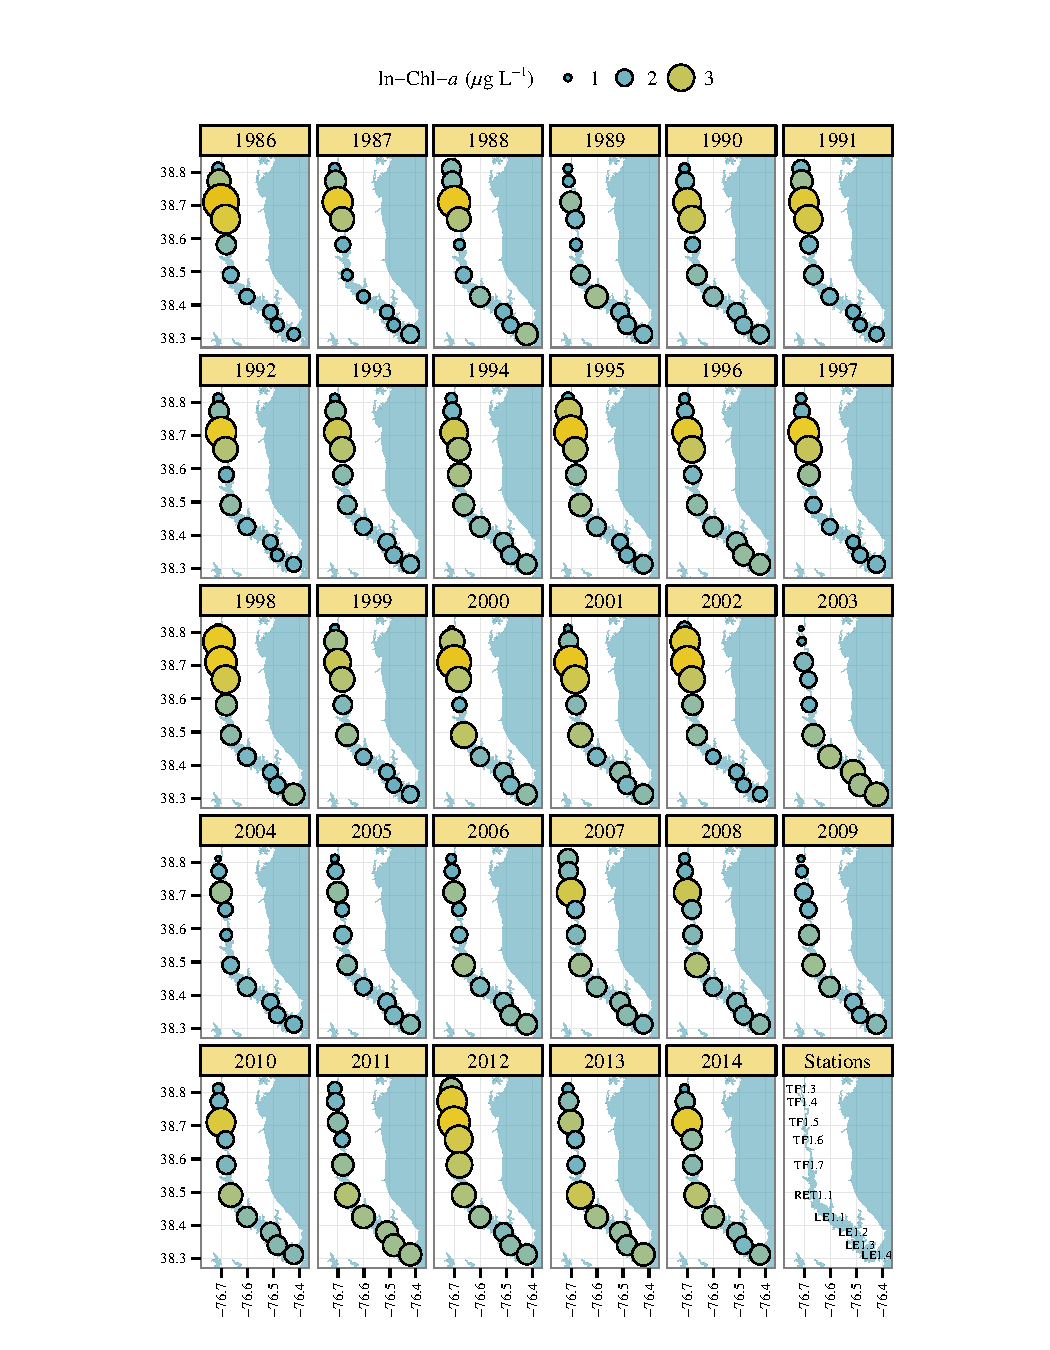
\includegraphics[width=\maxwidth]{figs/chlyr-1} 

}

\caption[Annual chlorophyll trends at each monitoring station in the Patuxent River Estuary]{Annual chlorophyll trends at each monitoring station in the Patuxent River Estuary.  Values are annual medians of ln-chlorophyll-a with size and color proportional between years.}\label{fig:chlyr}
\end{figure}



\begin{figure}[!ht]

{\centering 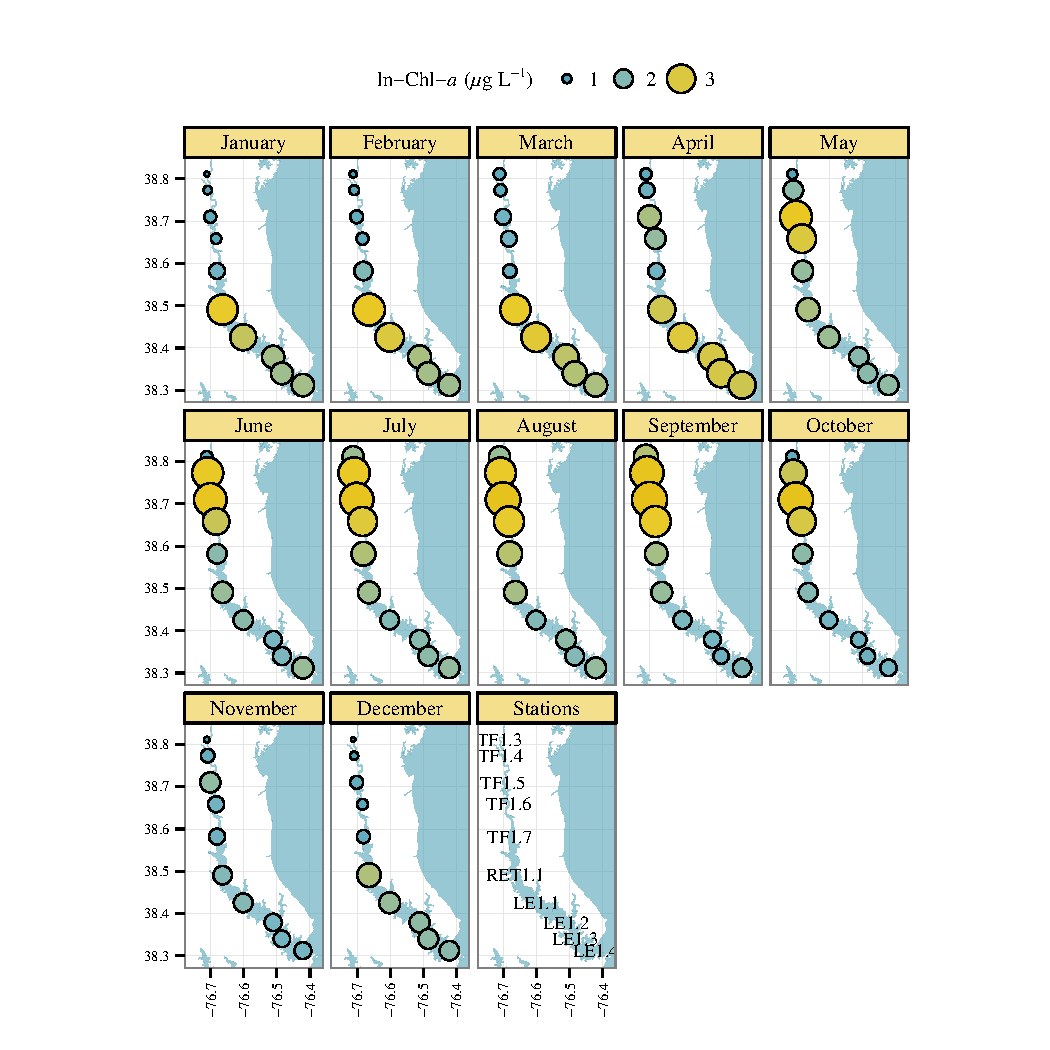
\includegraphics[width=\maxwidth]{figs/chlmo-1} 

}

\caption[Monthly chlorophyll trends at each monitoring station in the Patuxent River Estuary]{Monthly chlorophyll trends at each monitoring station in the Patuxent River Estuary.  Values are monthly medians of ln-chlorophyll-a with size and color proportional between months.}\label{fig:chlmo}
\end{figure}





\end{document}
